\newpage
\section{Questão 12-15}


\begin{figure}[H]
	\centering
	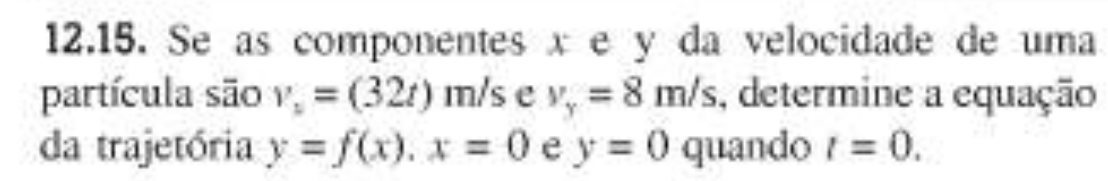
\includegraphics[width=.7\linewidth]{fundamentais/12-15.png}
	\caption{Comando da questão 12-15.}\label{fig:q12-15}
\end{figure}


Nesta questão, determinamos as equações paramétricas das posições \(x(t)\) e \(y(t)\), bem como a relação cartesiana entre as coordenadas \(x\) e \(y\), com base nos componentes da velocidade. A seguir, detalhamos o equacionamento.

\subsection*{Definição das Variáveis e Componentes de Velocidade}
As variáveis e os componentes da velocidade são definidos como:
\[
v_x = 32t, \quad v_y = 8,
\]
onde:
\begin{itemize}
    \item \(t\) representa o tempo;
    \item \(x\) e \(y\) representam as coordenadas no espaço.
\end{itemize}

\subsection*{Integração para Determinar as Posições em Função do Tempo}
A posição na direção \(x\) é obtida pela integração de \(v_x\):
\[
x(t) = \int v_x \, dt = \int 32t \, dt = 16t^2 + C_1.
\]

A posição na direção \(y\) é obtida pela integração de \(v_y\):
\[
y(t) = \int v_y \, dt = \int 8 \, dt = 8t + C_2.
\]

\subsection*{Determinação das Constantes de Integração}
Utilizando as condições iniciais:
\[
x(0) = 0 \quad \text{e} \quad y(0) = 0,
\]
determinamos as constantes \(C_1\) e \(C_2\):
\[
x(0) = 16(0)^2 + C_1 \implies C_1 = 0,
\]
\[
y(0) = 8(0) + C_2 \implies C_2 = 0.
\]

Substituindo as constantes nas equações, obtemos:
\[
x(t) = 16t^2, \quad y(t) = 8t.
\]

\subsection*{Eliminação de \(t\) para Determinar \(y\) em Função de \(x\)}
Da equação de \(x(t)\), resolvemos \(t\) em função de \(x\):
\[
x(t) = 16t^2 \implies t = \sqrt{\frac{x}{16}} = \frac{\sqrt{x}}{4}.
\]

Substituindo \(t\) na equação de \(y(t)\), obtemos:
\[
y = 8t = 8 \cdot \frac{\sqrt{x}}{4} = 2\sqrt{x}.
\]

Portanto, a equação cartesiana entre \(x\) e \(y\) é:
\[
y(x) = 2\sqrt{x}.
\]

\subsection*{Resultados Finais}
\begin{itemize}
    \item Equações paramétricas:
    \[
    x(t) = 16t^2, \quad y(t) = 8t.
    \]
    \item Relação cartesiana entre \(x\) e \(y\):
    \[
    y(x) = 2\sqrt{x}.
    \]
\end{itemize}
